\multiproblem{groups1}{Which of the following sets with binary operations are groups? Justify your answer. Here $+$ represents addition and $*$ denotes multiplication. (Note that you don't need to worry about the associativity because we have assumed this - see the preamble).
\begin{enumerate}
  \item $(\left\{ -1, 0, 1 \right\},+)$.
   \item $(\left\{-1, 0, 1 \right\},*)$.
  \item $(\left\{ -1, 1 \right\},*)$.
 \item $(\left\{ -1, 1 \right\},+)$.
   \item $(\left\{ -2,-1, 0, 1,2 \right\},+)$.
    \item $(\left\{ 3n : n\in \mathbb{Z} \right\},+)$.
    \item $(\left\{ 5^{n} : n\in \mathbb{Z} \right\},*)$.
\end{enumerate}
}

\multiproblem{groupsa}{Now we shall consider some groups of symmetries.
\begin{enumerate}
\item Consider the equilateral triangle shown below.\\
        \begin{center}
        \includegraphics[scale=1.5]{triangle.pdf}
        \end{center}
  It has the following three rotational symmetries:
  \begin{enumerate}
  \item $e$, the rotation of $0^{\circ}$ (doing nothing)
  \item $x$, the rotation of $120^{\circ}$ anticlockwise
  \item $y$, the rotation of $120^{\circ}$ clockwise.
  \end{enumerate}
  Now let $T=\left\{ e,x,y \right\}$ and $\bullet$ be the binary operation on $T$ such that $x\bullet y$ denotes transformation $y$ followed by transformation $x$. Find the table of $\bullet$ acting on the set $T$. Show that $(T,\bullet)$ a group. You can assume that $\bullet$ is associative. What is the identity element? What is the inverse of each element?
        \item
        Consider the square shown below.
                \begin{center}
        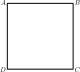
\includegraphics[scale=1.5]{square.pdf}
        \end{center}
        It has the following four rotational symmetries:
          \begin{enumerate}
  \item $e$, the rotation of $0^{\circ}$ (doing nothing)
  \item $x$, the rotation of $90^{\circ}$ anticlockwise
  \item $y$, the rotation of $180^{\circ}$
  \item $z$, the rotation of $90^{\circ}$ clockwise.
    \end{enumerate}
    Now let $S=\left\{ e,x,y,z \right\}$ and $\bullet$ be the associative binary operation as defined as in $(i)$. Find the table of $\bullet$ acting on the set $S$. Show that $(S,\bullet)$ a group. What is the identity element? What is the inverse of each element? There is one subgroup of order 2. Can you spot it?
    
        \item Consider the rectangle shown below.
                        \begin{center}
        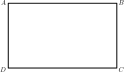
\includegraphics[scale=1.5]{rectangle.pdf}
        \end{center}
        It has the following flipping over symmetries:
        \begin{enumerate}
  \item $e$, not flipping (doing nothing)
  \item $h$, flipping horizontally
  \item $v$, flipping vertically
  \item $hv$, flipping vertically and then horizontally (note this is the same as $h\bullet v$).
  \end{enumerate}
        Now let $R=\left\{ e,h,v,hv \right\}$ and $\bullet$ be the associative binary operation as defined as in $(i)$. Find the table of $\bullet$ acting on the set $R$. Show that $(R,\bullet)$ a group. What is the identity element? What is the inverse of each element? There are three subgroups of order 2. Can you spot them?
        \end {enumerate}
}

\multiproblem{groupsb}{
\begin{enumerate}
 \item Show that $(\left\{0,1,2\right\},+\: \text{mod}\:3)$ is a group by finding the table of $+\: \text{mod} \:3$ over $\left\{0,1,2\right\}$. (Don't worry about associativity - you may assume modular addition is associative.) What is the identity element? What is the inverse of each element?
 \item Two finite groups are {\em isomorphic} if they have the same binary operation tables up to a relabelling of the elements. Compare the table you have just found in $(a)$ with that of the rotations of the triangle $(T,\bullet)$ in 2 (a). Are $(\left\{0,1,2\right\},+\: \text{mod}\: 3)$ and $(T,\bullet)$ isomorphic?
 \item Show that all groups of order 3 are isomorphic to one another. (Hint: Take a general set $e,x,y$ and binary operation. Consider what possible multiplication tables are possible whilst still keeping the group properties of closure, identity and inverse. It's a bit like completing a Sudoku.)
 \end{enumerate}
}

\multiproblem{groupsc}{
\begin{enumerate}
 \item Show that $(\left\{0,1,2,3\right\},+\: \text{mod}\: 4)$ is a group by finding the table of $+\: \text{mod}\: 4$ over $\left\{0,1,2,3\right\}$. What is the identity element? What is the inverse of each element? Which group in 2. is this group isomorphic to? 
 \item Show that $(\left\{1,3,5,7\right\},*\: \text{mod}\: 8)$ is a group by finding the table of $*\: \text{mod}\: 8$ over $\left\{1,3,5,7\right\}$. What is the identity element? What is the inverse of each element? (Don't worry about associativity - you may assume modular multiplication is associative.)  Which group in 2. is this group isomorphic to? 
 \item The group in (i) above is known as the cyclic group of order 4 (denoted $C_{4}$) and the group in (ii) is known as the Klein four-group (denoted $V_{4}$). Show that all groups of order 4 are isomorphic to one of these. (Hint: proceed in a similar way to 3 (iii).)
 \end{enumerate}
}

\multiproblem{groups2}{Now let us prove some properties that hold true for any group $(G,\bullet)$.
\begin{enumerate}
 \item Prove that $(x\bullet y)^{-1}=y^{-1}x^{-1}$  $\forall \: x,y\in G$.
 \item Prove that the identity element $e\in G$ is unique. 
 \item Prove that the inverse of any element $x^{-1}$ in $G$ is unique.
 \end {enumerate}
 Now suppose that $(G,\bullet)$ is an abelian group.
 \begin{enumerate}
 \item Prove that $(x\bullet y)^{2}=x^{2}\bullet y^{2}~~ \forall \: x,y \in G.$
\end{enumerate}
}

\multiproblem{groups}{
Which of the following infinite sets together with the associated binary operations are groups? If they are, are they Abelian? If they are groups, demonstrate that they are by showing that each of the conditions for a group holds. If they are not, justify by explaining which of the conditions is violated.
\begin{enumerate}
 \item $(\mathbb{Z},+)$.
 \item $(\mathbb{Z},-)$.
 \item $(\mathbb{C},+)$.
 \item $(\mathbb{N},-)$.
 \item $(\mathbb{Z} - \left\{ 2 \right\},+)$.
 \item $(2\mathbb{Z},+)$. Here $2\mathbb{Z}=\left\{2n:\:n\in \mathbb{Z} \right\}$, the set of even integers.
  \item $(\mathbb{Z} - 2\mathbb{Z},+)$.
 \item $(\mathbb{Q},+)$.
 \item $(\mathbb{Z} - \left\{ 0 \right\},*)$.
 \item $(\mathbb{Q},*)$.
  \item $(\mathbb{C} - \left\{0\right\} ,*)$, where $*$ represents complex multiplication.
 \item $(\left\{{\bf v}\in \mathbb{R}^{3}\right\},{{+}})$, where ${+}$ represents vector addition.
 \item $(\left\{ {\bf v} \in \mathbb{R}^{3} \right\},\cdot)$, where $\cdot$ represents the vector dot-product.
 \item $(\left\{{\bf v}\in \mathbb{R}^{3}\right\},{{\times}})$, where ${\times}$ represents the vector cross-product.
 \item $
        \left ( \left \{ \begin{pmatrix}
                 a & 0 \\
                 0 & b
                \end{pmatrix}
  :a,b\in\mathbb{R} \right \}, \times  \right  )
       $, where $\times$ represents matrix multiplication.
 \item $
        \left ( \left \{ \begin{pmatrix}
                 a & b \\
                 c & d
                \end{pmatrix}
  :a,b,c,d\in\mathbb{R}, ad \neq bc \right \}, \times \right)
       $, where $\times$ represents matrix multiplication.
       \item
       The set of all non-singular $n\times n$ matrices under matrix multiplication.
\end{enumerate}
}

